%\documentclass[a4paper]{article}
\usepackage[utf8]{inputenc}
\usepackage[spanish, es-tabla, es-noshorthands]{babel}
\usepackage[table,xcdraw]{xcolor}
\usepackage[a4paper, footnotesep = 1cm, width=22cm, top=2.5cm, height=25cm, textwidth=20cm, textheight=25cm]{geometry}
%\geometry{showframe}

\usepackage{tikz}
\usepackage{amsmath}
\usepackage{amsfonts}
\usepackage{amssymb}
\usepackage{float}
\usepackage{graphicx}
\usepackage{caption}
\usepackage{subcaption}
\usepackage{multicol}
\usepackage{multirow}
\usepackage{wrapfig}
\setlength{\doublerulesep}{\arrayrulewidth}
\usepackage{booktabs}

\usepackage{hyperref}
\hypersetup{
    colorlinks=true,
    linkcolor=blue,
    filecolor=magenta,      
    urlcolor=blue,
    citecolor=blue,    
}

\newcommand{\note}[1]{
	\begin{center}
		\huge{ \textcolor{red}{#1} }
	\end{center}
}

\setcounter{topnumber}{2}
\setcounter{bottomnumber}{2}
\setcounter{totalnumber}{4}
\renewcommand{\topfraction}{0.85}
\renewcommand{\bottomfraction}{0.85}
\renewcommand{\textfraction}{0.15}
\renewcommand{\floatpagefraction}{0.8}
\renewcommand{\textfraction}{0.1}
\setlength{\floatsep}{5pt plus 2pt minus 2pt}
\setlength{\textfloatsep}{5pt plus 2pt minus 2pt}
\setlength{\intextsep}{5pt plus 2pt minus 2pt}

\newcommand{\quotes}[1]{``#1''}
\usepackage{array}
\newcolumntype{C}[1]{>{\centering\let\newline\\\arraybackslash\hspace{0pt}}m{#1}}
\usepackage[american]{circuitikz}
\usetikzlibrary{calc}
\usepackage{fancyhdr}
\usepackage{units} 

\graphicspath{{../Ejercicio-1/}{../Ejercicio-2/}{../Ejercicio-3/}{../Ejercicio-4/}{../ParteI/}{../ParteII/}{../ParteIII/}{../ParteIV/}}

\pagestyle{fancy}
\fancyhf{}
\lhead{22.14 - Electrónica IV}
\rhead{Mechoulam, Lambertucci, Londero}
\rfoot{Página \thepage}

%
%\begin{document}

\subsection{Diseño del sistema}

Para el sistema que se busca desarrollar, se emplean los siguientes valores:
\begin{multicols}{2}
\begin{itemize}
	\item $D = 0.3$
	\item $L_1 = 40 \ \mu H$
	\item $R_1 = R_3 = 6.75 \ \Omega$
	\item $C_1 = C_3 = 47 \ \mu f$
	\item $C_2 = C_4 = 1 \ \mu f$
	\item $N_1 = 3 \ \mu H$
	\item $N_2 = N_3 = 1 \ \mu H$
\end{itemize}
\end{multicols}

\begin{figure}[H]
	\centering
	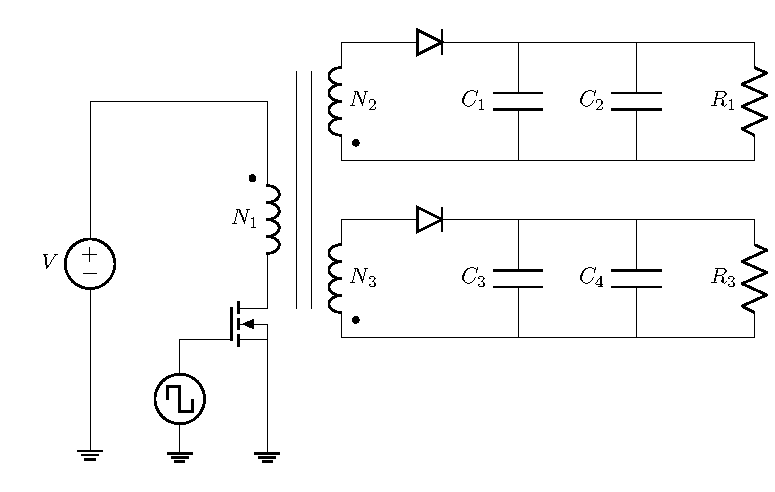
\includegraphics[width=0.7\linewidth, page = 1]{ImagenesParteII/Flyback.pdf}
	\label{fig:fly}
	\caption{Circuito del snubber empleado.}
\end{figure}

\subsection{Simulaciones}

Se simuló el circuito a lazo abierto. De esta forma se obtuvieron las siguientes curvas.
\begin{figure}[H]
	\centering
	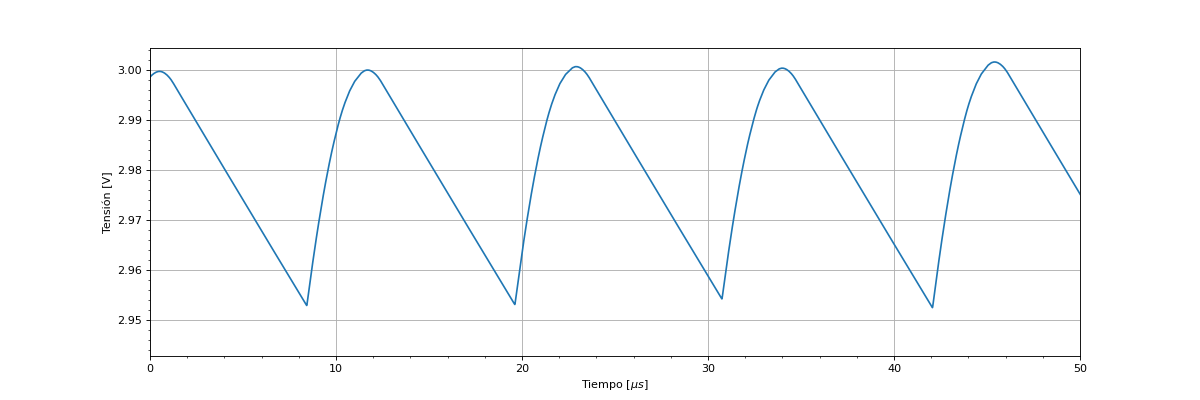
\includegraphics[width=0.9\linewidth]{ImagenesParteII/ Vo.png}
	\label{fig:vo}
	\caption{Tensión de salida.}
\end{figure}

\begin{figure}[H]
	\centering
	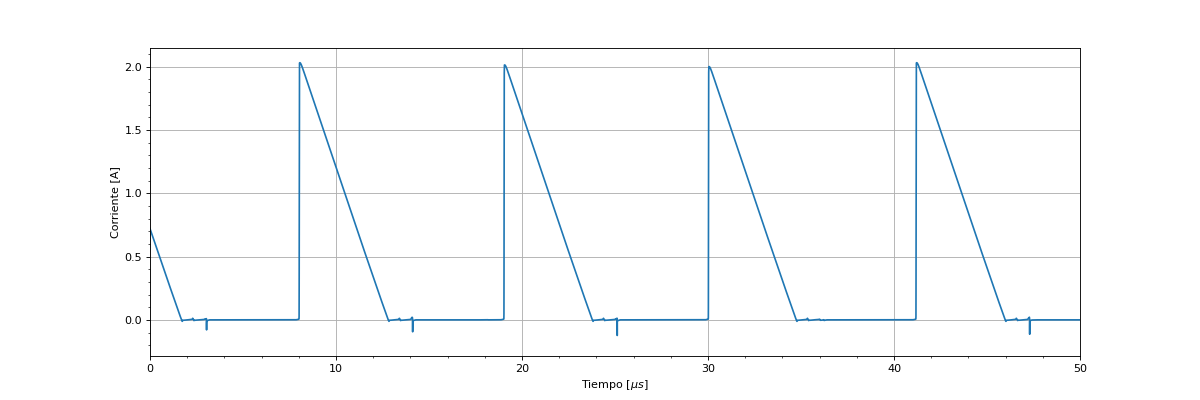
\includegraphics[width=0.9\linewidth]{ImagenesParteII/Idiodo.png}
	\label{fig:idiodo}
	\caption{Corriente del diodo.}
\end{figure}

\begin{figure}[H]
	\centering
	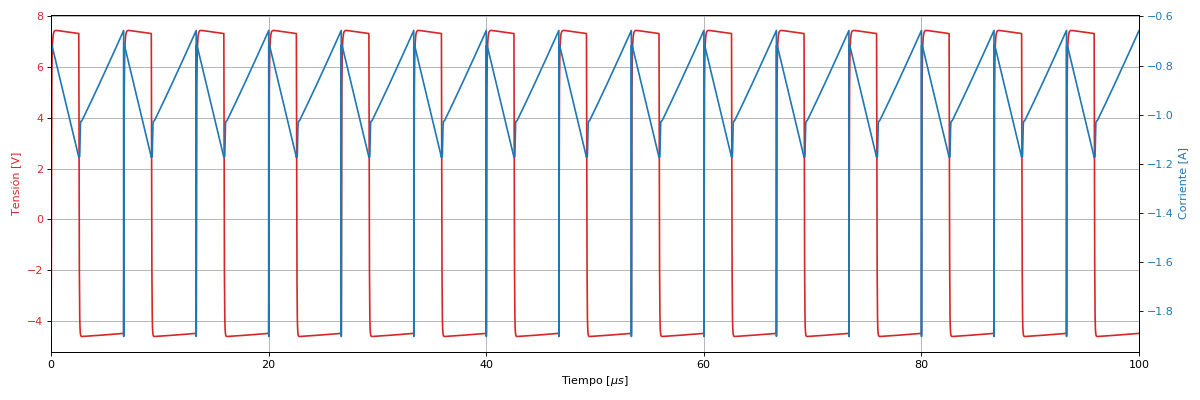
\includegraphics[width=0.9\linewidth]{ImagenesParteII/Primario.png}
	\label{fig:primario}
	\caption{Tensión y corriente del primario.}
\end{figure}

\begin{figure}[H]
	\centering
	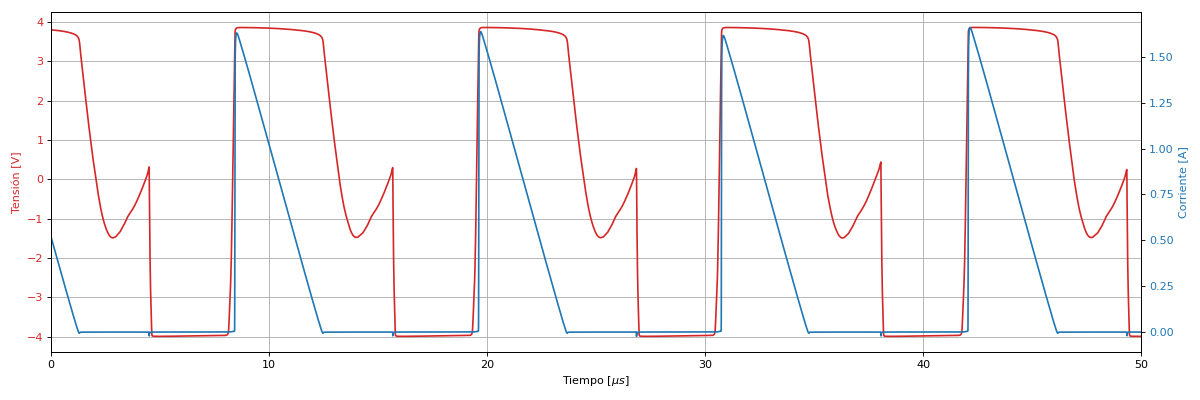
\includegraphics[width=0.9\linewidth]{ImagenesParteII/Secundario.png}
	\label{fig:secundario}
	\caption{Tensión y corriente del secundario.}
\end{figure}

\begin{figure}[H]
	\centering
	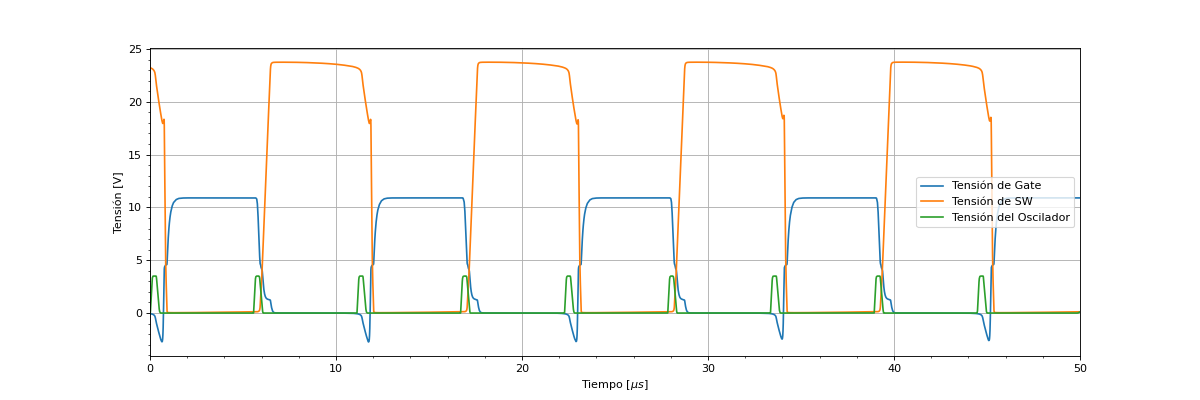
\includegraphics[width=0.9\linewidth]{ImagenesParteII/TensionesVarias1.png}
	\label{fig:tensionesvarias}
	\caption{Tensión de Gate y del Switch.}
\end{figure}

\subsection{Snubber}

Para el circuito dado, se diseña un snubber empleando un diodo, una resistencia y un capacitor.
\begin{figure}[H]
	\centering
	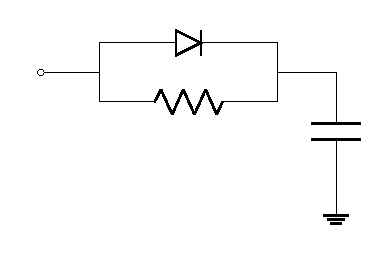
\includegraphics[width=0.3\linewidth, page = 1]{ImagenesParteII/Snubber.pdf}
	\label{fig:snubber}
	\caption{Circuito del snubber empleado.}
\end{figure}

Se calcula el valor máximo del capacitor, planteando que la energía de este debe ser mayor a la de la inductancia. De esta forma, se llega a la expresión:
\begin{equation}
	C > L_d \left( \frac{I_{L1}}{V_{C}} \right)^2 = 1 \ \mu H \cdot \left( \frac{15 \ A}{100 \ V} \right)^2 = 22.5 \ nF
\end{equation}

De esta forma, se selecciona $C = 10 \ nF$. Planteando que tres veces el tiempo característico del sistema RC debe ser menor al período de la fuente Flyback, se puede obtener una restricción similar para la resistencia. Operando, se llega a:
\begin{equation}
	R < \left. \frac{DT_S}{3C} \right|_{C = 10 \ nF} = \frac{0.5}{150 \ kHz} \cdot \frac{1}{3 \cdot 10 \ nF} = 111.11 \ \Omega
\end{equation}

Finalmente se selecciona $R = 47 \ \Omega$.

\begin{figure}[H]
	\centering
	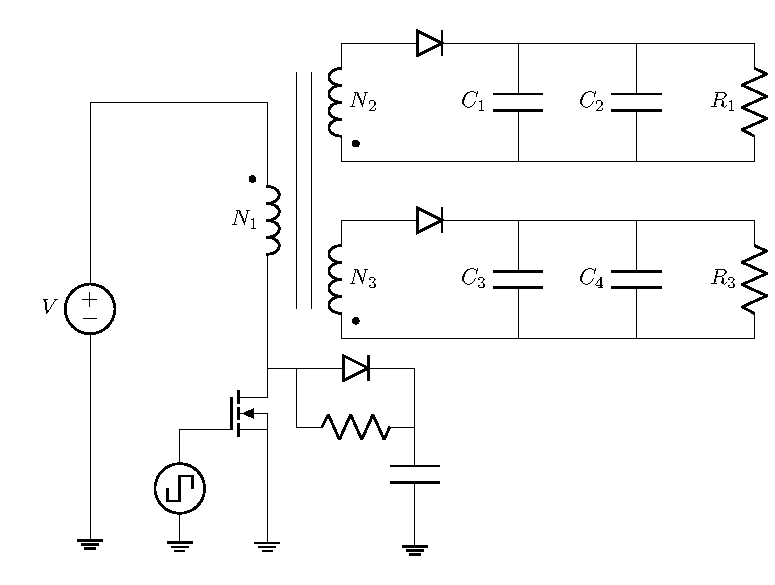
\includegraphics[width=0.7\linewidth, page = 1]{ImagenesParteII/FlybackSnubber.pdf}
	\label{fig:fly_snubber}
	\caption{Circuito Flyback con snubber.}
\end{figure}

%\end{document}